\documentclass[a4paper,ngerman]{tui-algo-seminar}
\usepackage{graphicx}
\usepackage{algorithm2e}
\usepackage{booktabs}
\usepackage{tikz}
\usepackage{hyperref}
\usepackage{caption}
\usepackage{float}
\usepackage{adjustbox}
\usepackage{listings}
\usepackage{totpages}  % Paket für die Gesamtseitenzahl
\setlength{\footskip}{13.0pt} % keine Ahnung ^^


\usepackage[utf8]{inputenc} % Verwenden Sie utf8 für UTF-8 Zeichencodierung

\newcommand{\inhalt}{8. Gerd Fornahl Turnier 2024}
\seminar{\inhalt}
\semester{\today}
\title{\inhalt}
\author{Erik Skopp}

\usepackage{fancyhdr}  % Für individuelle Kopf- und Fußzeilen
\nolinenumbers

% Definieren des Seitenstils
\pagestyle{fancy}
\fancyhf{}  % Vorherige Kopf- und Fußzeilen-Einstellungen löschen
%\fancyfoot[Rf]{\thepage ~von \zpageref{LastPage}}  % Gesamtseitenzahl
\begin{document}

\maketitle
\thispagestyle{plain} % Seitenzahl auf Seite 1 anzeigen
\begin{abstract}
Das Gerd-Fornahl-Gedenkturnier ehrt den einst führenden Spieler und Trainer des Ilmenauer Schachvereins und ist ein jährliches Event, das sein Vermächtnis in der Schachgemeinschaft fortleben lässt. Das 8. Turnier präsentierte eine vielfältige Teilnehmermischung, was für spannende Partien sorgte. Die erfolgreiche Durchführung wurde durch die Zusammenarbeit des Ilmenauer Schachvereins und des Vereins für Kulturelle Koordinierung ermöglicht. Trotz einiger Überraschungen bleibt die Atmosphäre des Turniers geprägt von Fairness, Leidenschaft und dem Geist des Schachs.
\end{abstract}

\tableofcontents 
\clearpage
\section{Wichtig. Bitte lesen}

Die Tabellen und Bilder hier können nur schwer in andere CMS und Medien integriert werden. Ich bitte daher dringend darum, die Bilder und Tabellen aus der Nextcloud des Ilmenauer Schachvereins zu verwenden. Die aktuellen URLs lauten wie folgt. Bitte beachten Sie, dass sich die URLs möglicherweise geändert haben, wenn Sie diesen Artikel lesen. Die Cloud unterliegt einem ständigen Wandel.
\begin{itemize}
    \item Bilder: \url{https://cloud.ilmenauer-schachverein.de/apps/files/files/89310?dir=/Events/2024_04_Gerd_Fornahl_Gedenkturnier_8/Bilder}
    \item Tabellen: \url{https://cloud.ilmenauer-schachverein.de/apps/files/files/89358?dir=/Events/2024_04_Gerd_Fornahl_Gedenkturnier_8/Tabellen}
\end{itemize}

Ich bitte außerdem darum, die Links zu den beiden Ergebnisdiensten zu integrieren. Dies verleiht nicht nur einen professionelleren Eindruck, sondern trägt auch wesentlich zur umfassenden Darstellung des Turniers bei.

\begin{itemize}
    \item Chess-Results: \url{https://chess-results.com/tnr923015.aspx?lan=0&art=9&fed=GER&turdet=YES&flag=30&snr=3}
     \item Find Chess Game: \url{https://www.findchessgames.com/index-0134,224,1131-turniere-anzeigen.html}
\end{itemize}
\clearpage
\section{Bericht}
\setlength{\parindent}{0pt}
Gerd Fornahl, einst führender Spieler und Trainer des Ilmenauer Schachvereins, prägte das Schachleben in Ilmenau nachhaltig durch seine herausragende Kinder- und Jugendarbeit. Nach seiner aktiven Zeit setzte er sein Engagement als Schiedsrichter und Trainer fort. Sein unerwarteter Tod hinterließ eine tiefe Lücke in der Schachgemeinschaft, die zu seinen Ehren das Gerd-Fornahl-Gedenkturnier ins Leben rief. ~\cite{fornahl2} ~\cite{fornahl1}

Das Teilnehmerfeld des 8. Gerd Fornahl Turniers präsentierte eine vielfältige Mischung aus Erfahrung und aufstrebendem Talent, angeführt von Ainur Ziganshin mit einer DWZ-Wertung von 2198. Mit Teilnehmern aus verschiedenen Ländern und Altersklassen versprach das Turnier spannende Partien. Besonders hervorzuheben waren die jungen Spieler wie Hai Phong Luu und die erfahrenen Spieler wie Torsten Michael, was die Breite des Teilnehmerfeldes unterstrich. Die starke Beteiligung des Ilmenauer Schachvereins betonte die lokale Verwurzelung der Veranstaltung.

Am 12. April 2024 ab 19:30 fand das 8. Gerd Fornahl Turnier im Ernst Abbe Zentrum der Technischen Universität Ilmenau statt. Diese Veranstaltung war nur durch die engagierte Zusammenarbeit des Ilmenauer Schachvereins und des Vereines für Kulturelle Koordinierung (Kukos) möglich, die gemeinsam eine ideale Plattform für das Turnier schufen.

Die ersten Runden des Turniers boten aufregende Duelle und zeigten einige klare Trends. Ainur Ziganshin und Uwe Mehlhorn starteten mit Siegen gegen Markus Hartung und Hanna Görlach. Marco Geißhirt, Stefan Schenk und Georg Lehmann setzten sich ebenfalls durch. Während Erik Skopp und Erik Heitmann ihre Partien gewannen, endete das Spiel zwischen Timo Jung und Torsten Michael unentschieden. Iresh Dudeja siegte gegen Jörg Peukert.

In den folgenden Runden setzten sich einige Spieler deutlich durch, während andere mit überraschenden Ergebnissen aufwarteten. Ainur Ziganshin behielt seine Dominanz bei und besiegte Uwe Mehlhorn. Marco Geißhirt gewann gegen Iresh Dudeja, während Timo Jung einen Sieg gegen Erik Heitmann einfuhr. Markus Hartung setzte sich gegen Markus Eisenbach durch, während Stefan Schenk Jörg Peukert besiegte. Georg Lehmann und Torsten Michael gewannen ebenfalls ihre Partien gegen Erik Skopp bzw. Ivan Krasnov. Hanna Görlach setzte sich gegen Hai Phong Luu durch, während Frank Winger Norik Lehmann besiegte.

Die späteren Runden sahen einige entscheidende Begegnungen, die das Gesamtbild des Turniers prägten. Ainur Ziganshin setzte seinen Lauf fort und besiegte Iresh Dudeja. Uwe Mehlhorn gewann gegen Erik Heitmann, während Marco Geißhirt Markus Hartung besiegte. Stefan Schenk setzte sich gegen Torsten Michael durch, während Georg Lehmann Markus Eisenbach bezwang. Timo Jung gewann gegen Jörg Peukert, Simon Greul besiegte Frank Winger, und Norik Lehmann gewann gegen Hanna Görlach. Erik Skopp triumphierte über Hai Phong Luu.

Die abschließende Runde des Turniers brachte die letzten Entscheidungen und krönte schließlich die Sieger. Ainur Ziganshin sicherte sich den Gesamtsieg, indem er Erik Heitmann besiegte. Uwe Mehlhorn gewann gegen Stefan Schenk, während Marco Geißhirt gegen Norik Lehmann siegte. Markus Hartung besiegte Timo Jung, Markus Eisenbach gewann gegen Iresh Dudeja, und Georg Lehmann setzte sich gegen Hai Phong Luu durch. Jörg Peukert besiegte Erik Skopp, Simon Greul gewann gegen Hanna Görlach, und Torsten Michael setzte sich gegen Frank Winger durch.

Nach 9 Runden waren Marco Geißhirt und Uwe Mehlhorn beide punktgleich und teilten sich den zweiten Platz. Um die Platzierung zu klären, einigten sich die beiden Spieler auf ein Stechen. Im Falle eines 1:1 wollte Uwe Marco den zweiten Platz überlassen, da dieser eine höhere Buchholz-Zahl hatte und es nicht zu einem Armageddon kommen sollte. In der ersten Partie gewann Uwe, nachdem Marco eine Remisstellung in eine verlorene Stellung umgewandelt hatte. In der zweiten Runde spielte Marco eine aggressive Variante und gewann mit einem starken Angriff. Somit stand es 1 zu 1, und Marco behielt seinen Platz auf dem zweiten Rang. ~\cite{marco1}

Bei der Siegerehrung des 8. Gerd Fornahl Gedenkturniers möchten wir unsere herausragenden Teilnehmer gebührend ehren. Ainur Ziganshin eroberte mit atemberaubender Leistung den ersten Platz, seine makellose Serie von 9 Siegen in 9 Runden ist ein wahrhaft bemerkenswerter Triumph. Herzlichen Glückwunsch zu diesem herausragenden Erfolg! Marco Geißhirt und Uwe Mehlhorn folgten dicht dahinter, sicherten sich den zweiten und dritten Platz mit bemerkenswerter Standhaftigkeit und beeindruckender Spielleistung.

Ein besonderer Applaus geht auch an Markus Hartung, Georg Lehmann und Dr. Markus Eisenbach, die sich mit beeindruckendem Können die Plätze vier, fünf und sechs sicherten und damit ihre Fähigkeiten unter Beweis stellten. Jedem Teilnehmer gebührt Anerkennung für seinen Einsatz und sein Engagement. Möge der Geist des Schachs weiterhin in ihnen brennen und sie zu weiteren Erfolgen inspirieren. Herzlichen Glückwunsch an alle!

Trotz der geringeren Teilnehmerzahlen wäre Gerd Fornahl zweifellos stolz auf das Turnier und die herausragende Leistung der Spieler. Sein Geist lebt weiter in jedem Zug, den sie machen. Wir blicken bereits gespannt auf das nächste Jahr, in dem wir erneut zusammenkommen werden, um sein Vermächtnis zu ehren und die Faszination des Schachs zu teilen.\vspace{1cm}

Erik Skopp\\
Ilmenauer Schachverein

\clearpage
\section{Tabellen}
\subsection{Links zu den Tabellen}
\begin{itemize}
    \item Chess-Result: \url{https://chess-results.com/Tnr923015.aspx?lan=0&art=1}
    \item Find Chess Game: \url{https://www.findchessgames.com/index-0134,224,1131-turniere-anzeigen.html}
\end{itemize}


Alle Tabellen stehen in der Cloud unter \url{https://cloud.ilmenauer-schachverein.de/apps/files/files/89358?dir=/Events/2024_04_Gerd_Fornahl_Gedenkturnier_8/Tabellen} zur Verfügung. Bitte nutzen Sie diese für die weitere Berichterstattung. 

\subsection{Startrangliste}
\begin{table}[H]
\centering
\caption{Teilnehmerliste: Sortiert nach Spielernummer}
\begin{tabular}{ccccccccc}
\hline
\textbf{TlnNr} & \textbf{Teilnehmer} & \textbf{ELO} & \textbf{NWZ} & \textbf{Verein/Ort} & \textbf{Land} & \textbf{Geburt} & \textbf{FideKenn} \\
\hline
1 & Ziganshin,Ainur & 1881 & 2198 & Ilmenauer SV & RUS & 1998 & 34111872 \\
2 & Mehlhorn,Uwe & 2019 & 1984 & SG Blau-Weiß Sta & GER & 1961 & 4619552 \\
3 & Geißhirt,Marco & 1965 & 1998 & SG Barchfeld/Bre & GER & 1990 & 4610563 \\
4 & Schenk,Stefan & 1993 & 1909 & Ilmenauer SV & GER & 1985 & 12924059 \\
5 & Lehmann,Georg & 1797 & 1585 & ESV Lok Meininge & GER & 2002 & 34613005 \\
6 & Skopp,Erik & 1710 & 1530 & Ilmenauer SV & GER & 1998 & 16201914 \\
7 & Michael,Torsten & & 1680 & Ilmenauer SV & GER & 1967 & 12982784 \\
8 & Heitmann,Erik & 1646 & 1587 & Erfurter SK & GER & 2012 & 34608940 \\
9 & Dudeja,Iresh & 1522 & 1587 & Ilmenauer SV & IND & 1992 & 25721380 \\
10 & Hartung,Markus & & 1584 & Ilmenauer SV & GER & 1987 & 16272510 \\
11 & Görlach,Hanna & 1578 & 1167 & Ilmenauer SV & GER & 2006 & 34675604 \\
12 & Eisenbach,Markus & & 1404 & Ilmenauer SV & GER & 1984 & 34663630 \\
13 & Krasnov,Ivan & & 1027 & Ilmenauer SV & RUS & 2009 & 55610650 \\
14 & Lehmann,Norik & & 970 & Ilmenauer SV & GER & 2010 & 34697195 \\
15 & Winger,Frank & & 838 & Ilmenauer SV & GER & 1964 & 16233069 \\
16 & Jung,Timo & & & Ilmenauer SV & GER & 2005 & \\
17 & Luu,Hai Phong & & & Ilmenauer SV & VIE & 2015 & \\
18 & Peukert, Jörg & & & & GER & 1974 & \\
19 & Greul,Simon & & & Ilmenauer SV & GER & 1998 & 34677577 \\
\hline
\end{tabular}
\end{table}


\clearpage


\subsection{Abschlusstabelle}
\begin{table}[H]
\centering
\caption{Rangliste: Stand nach der 9. Runde}
\begin{tabular}{cccccccccc}
\toprule
\textbf{Rang} & \textbf{Teilnehmer} & \textbf{TWZ} & \textbf{Verein/Ort} & \textbf{Land} & \textbf{S} & \textbf{R} & \textbf{V} & \textbf{Punkte} & \textbf{Buchh} \\
\midrule
1  & Ziganshin, Ainur     & 1881 & Ilmenauer SV      & RUS & 9 & 0 & 0 & 9.0 & 44.5  \\
2  & Geißhirt, Marco      & 1965 & SG Barchfeld/Br   & GER & 7 & 1 & 1 & 7.5 & 48.5  \\
3  & Mehlhorn, Uwe        & 2019 & SG Blau-Weiß St   & GER & 7 & 1 & 1 & 7.5 & 45.5  \\
4  & Hartung, Markus      & 1584 & Ilmenauer SV      & GER & 5 & 1 & 3 & 5.5 & 52.5  \\
5  & Lehmann, Georg       & 1797 & ESV Lok Meining   & GER & 5 & 0 & 4 & 5.0 & 39.5  \\
6  & Eisenbach, Markus    & 1404 & Ilmenauer SV      & GER & 4 & 2 & 3 & 5.0 & 36.0  \\
7  & Heitmann, Erik       & 1646 & Erfurter SK       & GER & 4 & 1 & 4 & 4.5 & 46.5  \\
8  & Peukert, Jörg        &      &                   & GER & 4 & 1 & 4 & 4.5 & 32.0  \\
9  & Dudeja, Iresh        & 1522 & Ilmenauer SV      & IND & 4 & 0 & 5 & 4.0 & 49.5  \\
10 & Schenk, Stefan       & 1993 & Ilmenauer SV      & GER & 3 & 2 & 4 & 4.0 & 49.0  \\
11 & Jung, Timo           &      & Ilmenauer SV      & GER & 3 & 2 & 4 & 4.0 & 45.0  \\
12 & Michael, Torsten     & 1680 & Ilmenauer SV      & GER & 3 & 2 & 4 & 4.0 & 38.5  \\
13 & Lehmann, Norik       & 970  & Ilmenauer SV      & GER & 4 & 0 & 5 & 4.0 & 34.5  \\
14 & Greul, Simon         &      & Ilmenauer SV      & GER & 4 & 0 & 5 & 4.0 & 30.5  \\
15 & Skopp, Erik          & 1710 & Ilmenauer SV      & GER & 3 & 1 & 5 & 3.5 & 35.5  \\
16 & Görlach, Hanna       & 1578 & Ilmenauer SV      & GER & 2 & 0 & 7 & 2.0 & 35.5  \\
17 & Winger, Frank        & 838  & Ilmenauer SV      & GER & 2 & 0 & 7 & 2.0 & 34.0  \\
18 & Krasnov, Ivan        & 1027 & Ilmenauer SV      & RUS & 1 & 0 & 8 & 1.0 & 27.5  \\
19 & Luu, Hai Phong       &      & Ilmenauer SV      & VIE & 0 & 0 & 9 & 0.0 & 35.5  \\
\bottomrule
\end{tabular}
\end{table}




\section{Paarungen}
\subsection{Runde 1}
\begin{table}[H]
\centering
\caption{Paarungsliste der 1. Runde des 8. Gerd Fornahl Gedenkturniers}
\begin{tabular}{cllcl}
\toprule
\textbf{Tisch} & \textbf{Weiß} & \textbf{Schwarz} & \textbf{Ergebnis} \\
\midrule
1 & Hartung, Markus & Ziganshin, Ainur & 0 - 1 \\
2 & Mehlhorn, Uwe & Görlach, Hanna & 1 - 0 \\
3 & Eisenbach, Markus & Geißhirt, Marco & 0 - 1 \\
4 & Schenk, Stefan & Krasnov, Ivan & 1 - 0 \\
5 & Lehmann, Norik & Lehmann, Georg & 0 - 1 \\
6 & Skopp, Erik & Winger, Frank & 1 - 0 \\
7 & Jung, Timo & Michael, Torsten & ½ - ½ \\
8 & Heitmann, Erik & Luu, Hai Phong & 1 - 0 \\
9 & Peukert, Jörg & Dudeja, Iresh & 0 - 1 \\
\bottomrule
\end{tabular}
\end{table}

\subsection{Runde 2}
\begin{table}[H]
\centering
\caption{Paarungsliste der 2. Runde des 8. Gerd Fornahl Gedenkturniers}
\begin{tabular}{cllcl}
\toprule
\textbf{Tisch} & \textbf{Weiß} & \textbf{Schwarz} & \textbf{Ergebnis} \\
\midrule
1 & Ziganshin, Ainur & Skopp, Erik & 1 - 0 \\
2 & Lehmann, Georg & Mehlhorn, Uwe & 0 - 1 \\
3 & Geißhirt, Marco & Heitmann, Erik & 1 - 0 \\
4 & Dudeja, Iresh & Schenk, Stefan & 1 - 0 \\
5 & Michael, Torsten & Hartung, Markus & 0 - 1 \\
6 & Görlach, Hanna & Jung, Timo & 0 - 1 \\
7 & Winger, Frank & Eisenbach, Markus & 0 - 1 \\
8 & Krasnov, Ivan & Peukert, Jörg & 0 - 1 \\
9 & Luu, Hai Phong & Lehmann, Norik & 0 - 1 \\
\bottomrule
\end{tabular}
\end{table}

\subsection{Runde 3}
\begin{center}
\captionof{table}{Paarungsliste der 3. Runde des 8. Gerd Fornahl Gedenkturniers}
\begin{tabular}{cllcl}
\toprule
\textbf{Tisch} & \textbf{Weiß} & \textbf{Schwarz} & \textbf{Ergebnis} \\
\midrule
1 & Geißhirt, Marco & Ziganshin, Ainur & 0 - 1 \\
2 & Mehlhorn, Uwe & Dudeja, Iresh & 1 - 0 \\
3 & Jung, Timo & Schenk, Stefan & ½ - ½ \\
4 & Hartung, Markus & Lehmann, Georg & 1 - 0 \\
5 & Skopp, Erik & Eisenbach, Markus & ½ - ½ \\
6 & Heitmann, Erik & Lehmann, Norik & 1 - 0 \\
7 & Peukert, Jörg & Michael, Torsten & ½ - ½ \\
8 & Winger, Frank & Görlach, Hanna & 0 - 1 \\
9 & Luu, Hai Phong & Krasnov, Ivan & 0 - 1 \\
\bottomrule
\end{tabular}
\end{center}

\subsection{Runde 4}
\begin{center}
\captionof{table}{Paarungsliste der 4. Runde des 8. Gerd Fornahl Gedenkturniers}
\begin{tabular}{cllcl}
\toprule
\textbf{Tisch} & \textbf{Weiß} & \textbf{Schwarz} & \textbf{Ergebnis} \\
\midrule
1 & Ziganshin, Ainur & Mehlhorn, Uwe & 1 - 0 \\
2 & Dudeja, Iresh & Geißhirt, Marco & 0 - 1 \\
3 & Jung, Timo & Heitmann, Erik & 1 - 0 \\
4 & Eisenbach, Markus & Hartung, Markus & 0 - 1 \\
5 & Schenk, Stefan & Peukert, Jörg & 1 - 0 \\
6 & Lehmann, Georg & Skopp, Erik & 1 - 0 \\
7 & Michael, Torsten & Krasnov, Ivan & 1 - 0 \\
8 & Görlach, Hanna & Luu, Hai Phong & 1 - 0 \\
9 & Lehmann, Norik & Winger, Frank & 0 - 1 \\
\bottomrule
\end{tabular}
\end{center}
\clearpage

\subsection{Runde 5}
\begin{center}
\captionof{table}{Paarungsliste der 5. Runde des 8. Gerd Fornahl Gedenkturniers}
\begin{tabular}{cllcl}
\toprule
\textbf{Tisch} & \textbf{Weiß} & \textbf{Schwarz} & \textbf{Ergebnis} \\
\midrule
1 & Ziganshin, Ainur & Jung, Timo & 1 - 0 \\
2 & Mehlhorn, Uwe & Hartung, Markus & 1 - 0 \\
3 & Geißhirt, Marco & Schenk, Stefan & 1 - 0 \\
4 & Heitmann, Erik & Lehmann, Georg & 1 - 0 \\
5 & Görlach, Hanna & Michael, Torsten & 0 - 1 \\
6 & Skopp, Erik & Dudeja, Iresh & 0 - 1 \\
7 & Peukert, Jörg & Eisenbach, Markus & 0 - 1 \\
8 & Greul, Simon & Lehmann, Norik & 1 - 0 \\
9 & Winger, Frank & Luu, Hai Phong & 1 - 0 \\
\bottomrule
\end{tabular}
\end{center}

\subsection{Runde 6}
\begin{center}
\captionof{table}{Paarungsliste der 6. Runde des 8. Gerd Fornahl Gedenkturniers}
\begin{tabular}{cllcl}
\toprule
\textbf{Tisch} & \textbf{Weiß} & \textbf{Schwarz} & \textbf{Ergebnis} \\
\midrule
1 & Michael, Torsten & Ziganshin, Ainur & 0 - 1 \\
2 & Mehlhorn, Uwe & Geißhirt, Marco & ½ - ½ \\
3 & Hartung, Markus & Heitmann, Erik & ½ - ½ \\
4 & Dudeja, Iresh & Jung, Timo & 1 - 0 \\
5 & Schenk, Stefan & Eisenbach, Markus & ½ - ½ \\
6 & Lehmann, Georg & Winger, Frank & 1 - 0 \\
7 & Peukert, Jörg & Görlach, Hanna & 1 - 0 \\
8 & Lehmann, Norik & Skopp, Erik & 1 - 0 \\
9 & Luu, Hai Phong & Greul, Simon & 0 - 1 \\
\bottomrule
\end{tabular}
\end{center}

\subsection{Runde 7}
\begin{center}
\captionof{table}{Paarungsliste der 7. Runde des 8. Gerd Fornahl Gedenkturniers}
\begin{tabular}{cllcl}
\toprule
\textbf{Tisch} & \textbf{Weiß} & \textbf{Schwarz} & \textbf{Ergebnis} \\
\midrule
1 & Ziganshin, Ainur & Dudeja, Iresh & 1 - 0 \\
2 & Heitmann, Erik & Mehlhorn, Uwe & 0 - 1 \\
3 & Geißhirt, Marco & Hartung, Markus & 1 - 0 \\
4 & Schenk, Stefan & Michael, Torsten & 1 - 0 \\
5 & Eisenbach, Markus & Lehmann, Georg & 0 - 1 \\
6 & Jung, Timo & Peukert, Jörg & 1 - 0 \\
7 & Greul, Simon & Winger, Frank & 1 - 0 \\
8 & Görlach, Hanna & Lehmann, Norik & 0 - 1 \\
9 & Skopp, Erik & Luu, Hai Phong & 1 - 0 \\
\bottomrule
\end{tabular}
\end{center}
\clearpage

\subsection{Runde 8}
\begin{center}
\captionof{table}{Paarungsliste der 8. Runde des 8. Gerd Fornahl Gedenkturniers}
\begin{tabular}{cllcl}
\toprule
\textbf{Tisch} & \textbf{Weiß} & \textbf{Schwarz} & \textbf{Ergebnis} \\
\midrule
1 & Ziganshin, Ainur & Schenk, Stefan & 1 - 0 \\
2 & Mehlhorn, Uwe & Jung, Timo & 1 - 0 \\
3 & Lehmann, Georg & Geißhirt, Marco & 0 - 1 \\
4 & Dudeja, Iresh & Heitmann, Erik & 0 - 1 \\
5 & Hartung, Markus & Greul, Simon & 1 - 0 \\
6 & Lehmann, Norik & Michael, Torsten & 1 - 0 \\
7 & Luu, Hai Phong & Eisenbach, Markus & 0 - 1 \\
8 & Skopp, Erik & Görlach, Hanna & 1 - 0 \\
9 & Winger, Frank & Peukert, Jörg & 0 - 1 \\
\bottomrule
\end{tabular}
\end{center}


\subsection{Runde 9}
\begin{center}
\captionof{table}{Paarungsliste der 9. Runde des 8. Gerd Fornahl Gedenkturniers}
\begin{tabular}{cllcl}
\toprule
\textbf{Tisch} & \textbf{Weiß} & \textbf{Schwarz} & \textbf{Ergebnis} \\
\midrule
1 & Heitmann, Erik & Ziganshin, Ainur & 0 - 1 \\
2 & Schenk, Stefan & Mehlhorn, Uwe & 0 - 1 \\
3 & Geißhirt, Marco & Lehmann, Norik & 1 - 0 \\
4 & Jung, Timo & Hartung, Markus & 0 - 1 \\
5 & Eisenbach, Markus & Dudeja, Iresh & 1 - 0 \\
6 & Luu, Hai Phong & Lehmann, Georg & 0 - 1 \\
7 & Peukert, Jörg & Skopp, Erik & 1 - 0 \\
8 & Greul, Simon & Görlach, Hanna & 1 - 0 \\
9 & Michael, Torsten & Winger, Frank & 1 - 0 \\
\bottomrule
\end{tabular}
\end{center}
\clearpage

\section{Bilder}
Alle Bilder stehen in der Cloud unter \url{https://cloud.ilmenauer-schachverein.de/apps/files/files/89310?dir=/Events/2024_04_Gerd_Fornahl_Gedenkturnier_8/Bilder} zur Verfügung. Bitte nutzen Sie diese für die weitere Berichterstattung.

\subsection{Siegerehrung Bild 1}
\begin{center}
    \adjustbox{width=\linewidth,height=0.5625\linewidth,keepaspectratio}{\includegraphics{2024_04_Gerd_Fornahl_Gedenkturnier_8_01}}
    \captionof{figure}{Siegerehrung Bild 1}
    \label{fig:gerd_fornahl_1}
\end{center}

\clearpage

\subsection{Siegerehrung Bild 2}
\begin{center}
    \adjustbox{width=\linewidth,height=0.5625\linewidth,keepaspectratio}{\includegraphics{2024_04_Gerd_Fornahl_Gedenkturnier_8_02}}
    \captionof{figure}{Siegerehrung Bild 2}
    \label{fig:gerd_fornahl_2}
\end{center}

\clearpage

\subsection{Siegerehrung Bild 3}
\begin{center}
    \adjustbox{angle=270,keepaspectratio}{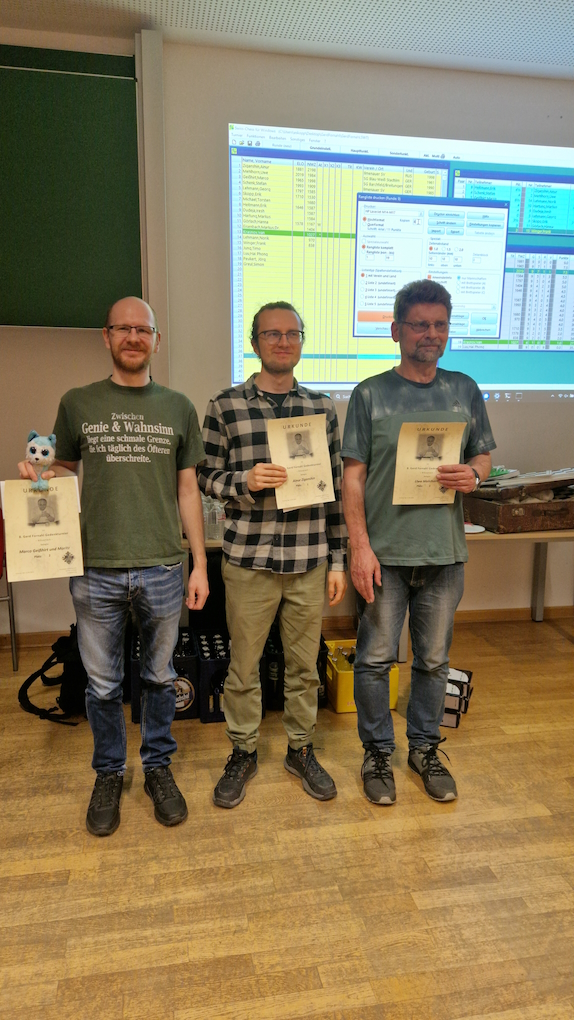
\includegraphics{2024_04_Gerd_Fornahl_Gedenkturnier_8_03}}
    \captionof{figure}{Siegerehrung Bild 3}
    \label{fig:gerd_fornahl_3}
\end{center}

\clearpage

\subsection{Siegerehrung Bild 4}
\begin{center}
    \adjustbox{width=\linewidth,height=0.5625\linewidth,keepaspectratio}{\includegraphics{2024_04_Gerd_Fornahl_Gedenkturnier_8_04}}
    \captionof{figure}{Siegerehrung Bild 4}
    \label{fig:gerd_fornahl_4}
\end{center}

\clearpage
\section{Anhang}
\bibliography{2024_04_Gerd_Fornahl_Gedenkturnier_8/literatur}
%\listoffigures
%\listoftables

\end{document}
